\chapter{Introducción}

\section{Motivación y análisis del problema}
\bigskip
Como ya hemos hablado en el capítulo anterior, {\titulo} viene de una aplicación móvil híbrida en la que se detectaron carencias que probablemente provengan de la inexperiencia y el escaso tiempo de análisis del que se disponía. Vamos a exponer brevemente las características de las aplicaciones híbridas para entender los problemas que este proyecto pretende solventar.

\subsection{Aplicaciones móviles híbridas}
Con la llegada de los \textit{smartphone} se ha impulsado enormemente el consumo y producción de apps móviles. En un principio, una aplicación móvil se desarrollaba como aplicación nativa con los contras que ello supone, como una curva de aprendizaje alta de un sistema concreto, en la mayoría de los casos desarrollo monoplataforma, y también los pros como un desarrollo y control mas específico del sistema, sistemas mas robustos,etc.

\bigskip
Ni que decir tiene que una aplicación compleja necesita las ventajas de un desarrollo específico y nativo de un sistema móvil, pero ¿qué pasa con las aplicaciones simples y livianas que, cada vez más, consumimos? Es aquí donde toman importancia las aplicaciones móviles híbridas.

\begin{figure}[!ht]
  \begin{center}
  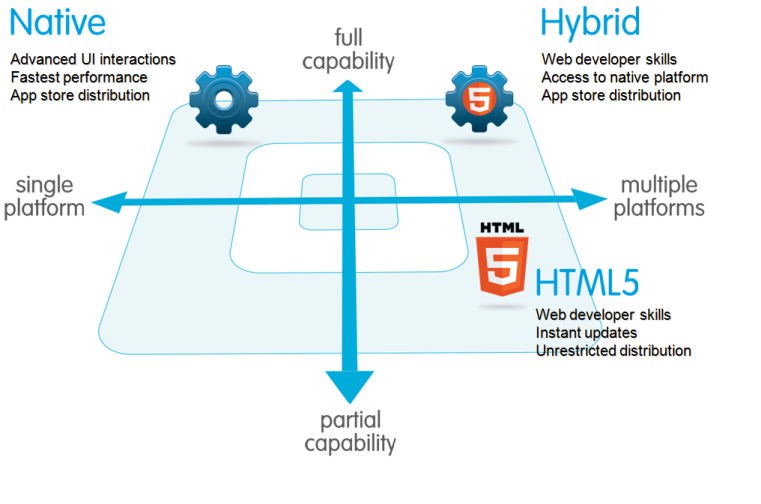
\includegraphics[width=0.9\textwidth]{../images/compare_hybrid_app.png}
  \caption[App híbrida]{App móvil híbrida (\href{https://developer.salesforce.com}{https://developer.salesforce.com}).}
  \label{fig:compare_hybrid_app}
  \end{center}
\end{figure}

Las principales ventajas de estas aplicaciones son:

\begin{itemize}
  \item \itembf{Bajo coste de desarrollo.}
  \item \itembf{Multiplataforma.}
  \item \itembf{Tiempo de desarrollo corto.}
  \item \itembf{Fácil distribución.}
\end{itemize}


\bigskip
Y lo que más nos interesa para este proyecto, sus desventajas:

\begin{itemize}
  \item \itembf{Rendimiento pobre.}
  \item \itembf{Escalabilidad baja.}
  \item \itembf{Diseño sujeto al diseño web.}
  \item \itembf{Acceso a las características especiales del hardware limitado.}
\end{itemize}


\bigskip
En un principio la aplicación que se desarrolló en el período de prácticas ICARO se planteó como una aplicación sencilla donde consultar conceptos y esquemas de las asignaturas. Los datos se consultarían desde una hoja de Google Drive común al departamento y se mostrarían en la aplicación directamente y por estas características, se .

A medida que avanzaba el desarrollo  y acercándose la fase final, el ``cliente'' planteó nuevas funcionalidades, topándonos con el primer problema: \textbf{la escalabilidad} de estas aplicaciones.



\subsection{Análisis del problema}
Una vez desarrollada esta aplicación, aunque en general quedamos contentos con el resultado, acusamos los siguientes problemas:

\begin{itemize}
  \item \itembf{No disponíamos de un servidor, toda la aplicación se ejecutaba en el cliente.}
  \item \itembf{Falta de base de datos.}
  \item \itembf{No se usa la API de Google Drive}
  \item \itembf{Acceso a Google Drive en cada sección de la aplicación}
  \item \itembf{Lentitud de acceso de datos en cada sección de la aplicación}
  \item \itembf{Mala elección de framework CSS, señales de obsoleto.}
\end{itemize}

\bigskip 
Solventar estos problemas, con el fin de iniciar un proyecto mejor planificado, con miras a una mayor escalabilidad analizando los requisitos presentes y los que pudieran surgir en un futuro, es la principal motivación para este proyecto. Aprovecharemos para mejorar la experiencia de usuario, ya que la lentitud de carga entre secciones era uno de los grandes problemas que hacían tediosa la consulta del contenido de la asignatura.

\bigskip
El primer paso importante es olvidar la tecnología móvil híbrida, que originó muchos problemas en el proyecto anterior y dividirlo en dos, una parte de desarrollo web y una parte de desarrollo móvil capaces de escalar sin problema. Nuestro proyecto se centrará en la aplicación web.


\section{Estado del arte y elección de la tecnología}
Para abordar los problemas descritos y antes de realizar un análisis más profundo se hará un estudio de las tecnologías web que pueden sernos útiles en proyectos de este tipo. Teniendo claro que vamos a desarrollar el proyecto bajo una arquitectura web y hecho el repaso de los inconvenientes en las tecnologías híbridas podemos sintetizar los siguientes puntos que necesita nuestro nuevo proyecto:

\begin{itemize}
  \item \itembf{Servir el contenido con un servidor web.}
  \item \itembf{Consultar el contenido de la hoja de Google Drive del Departamento.}
  \item \itembf{Almacenar el contenido en una base de datos.}
  \item \itembf{Gestión de usuarios.}
  \item \itembf{Establecer roles para los usuarios.}
\end{itemize}

\subsection{El lenguaje de programación}

\bigskip 
Lo primero que vamos a plantearnos es el \textbf{lenguaje} a usar, y que mejor forma de abrir un abanico de posibilidades que explorar los lenguajes más usados en la comunidad de GitHub\footnote{GitHub es una plataforma de desarrollo colaborativo donde usted puede alojar proyectos propios así como contribuir en otros proyectos. GitHub usa el sistema de control de versiones Git.} desde mediados de 2016 a mediados de 2017.

\begin{figure}[!ht]
  \begin{center}
  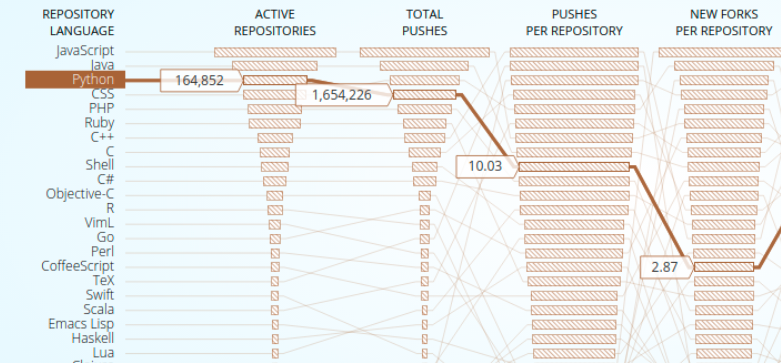
\includegraphics[width=1\textwidth]{../images/trend_lang_github_16-17.png}
  \caption[Top languages GitHub]{Top languages GitHub (\href{http://githut.info/}{http://githut.info/}).}
  \label{fig:trending_languages_github_16-17}
  \end{center}
\end{figure}

\bigskip
Como podemos ver en la figura anterior, entre los 5 lenguajes más usados se encuentran: JavaScript, Java, Python, PHP y Ruby (y sí, está CSS y lo hemos obviado ya que es un lenguaje usado únicamente para definir los estilos de un documenta HTML o XML). 

\bigskip
\textbf{JavaScript} nos ofrece la alternativa de Node.js para el lado del servidor pero no está diseñado para aplicaciones complejas. Node.js es un lenguaje interpretado y aunque trabaja de forma asíncrona, está diseñado para ejecutarse en un sólo hilo, por lo que podría presentar ciertas limitaciones a la hora de escalar en aplicaciones complejas. Además las aplicaciones con Node.js permanecen en RAM, no siendo re-interpretadas con nuevas peticiones si no que se procesa directamente desde la memoria.

\bigskip
JavaScript no se estudió profundamente durante el {\grado} y aunque descubrir e indagar en un lenguaje nuevo podría ser un aliciente, sus propiedades y las ``limitaciones'' en cuanto a la escalabilidad, que recuerdan al desarrollo en JavaScript de las aplicaciones híbridas, nos hacen descartar este lenguaje.

\bigskip
\textbf{Java} en cambio es un lenguaje que hemos profundizado más durante los años de estudio. Si es verdad que la mayoría del desarrollo que llevamos a cabo estos años era referente a aplicaciones de escritorio, pero la idea de un lenguaje nuevo o poco profundizado nos parecía más interesante en este proyecto.

\bigskip
Llegamos a los tres lenguajes que nos parecieron más interesantes para el proyecto \textbf{PHP}, \textbf{Ruby} y \textbf{Python}\cite{python_blackbook}. A una primera vista estos lenguajes eran candidatos para el desarrollo, vamos a señalar las características que se observaron para decidirnos por uno:


\bigskip
\begin{table}[htb]
\begin{tabular}{| p{4.2cm}| p{4.2cm} | p{4.2cm} |}
\hline
\multicolumn{3}{|c|}{\textbf{Características}} \\
\hline
\textbf{PHP} & \textbf{Ruby} & \textbf{Python} \\
\hline \hline \hline

Curva de aprendizaje corta & Curva de aprendizaje compleja & Curva de aprendizaje corta\\ \hline
Legibilidad y estructuración baja & Legibilidad y estructuración media & Legibilidad y estructuración alta \\ \hline
Popularidad alta & Popularidad baja & Popularidad media \\ \hline
Comunidad media & Comunidad media & Comunidad alta \\ \hline
\end{tabular}
\caption{Tabla de características.}
\label{tabla:anchofijo}
\end{table}

\bigskip
Hemos visto que PHP es el más usado en cuanto a cantidad de aplicaciones totales desarrolladas, pero a lo largo del último año, como se aprecia en la figura \ref{fig:trending_languages_github_16-17}, Python ha crecido enormemente en el número de contribuciones y en su comunidad. Viendo la evolución de este lenguaje y teniendo en cuenta sus características que ayudan a crear aplicaciones bien estructuradas, escalables, con módulos altamente reutilizables y teniendo una comunidad, tanto anglosajona como hispana, tan grande, Python será la opción elegida como lenguaje de \titulo .

\bigskip
Decir también que durante el grado se hizo una breve introducción a Python y se usó para pequeñas y aisladas aplicaciones, sintiendo una gran inquietud por usar este lenguaje en un proyecto más completo.




\subsection{Framework web}

Un framework web\cite{python_wiki, django_basic} es una colección de paquetes o módulos que permiten a los desarrolladores escribir aplicaciones o servicios web sin tener que manejar detalles de bajo nivel como protocolos, sockets o gestión de procesos.

\bigskip
Las aplicaciones web comúnmente utilizan y hacen uso de una serie de componentes, ya sea durante su desarrollo o en la etapa de producción, tales como un servidor HTTP, mecanismos de almacenamiento como podría ser una base de datos, un motor de plantillas, un conjunto de herramientas AJAX, etc. Estos framework agrupan y gestionan paquetes con estos componentes que ayudan en la abstracción del desarrollo de bajo nivel.

\bigskip
Ya que tenemos claro el lenguaje, vamos a hacer un breve estudio de los frameworks web existentes que nos permitirán un desarrollo ágil y mejor estructurado. Los tres frameworks web más importantes de Python por su volumen de proyectos, comunidad y completitud son:


\begin{itemize}
  \item {Django}
  \item {TurboGears2}
  \item {Web2Py}
\end{itemize}


\bigskip
Entre ellos, \textbf{Django}\cite{django_basic} es claramente el más usado y con una comunidad más grande. Se basa en el principio DRY\footnote{Don't Repeat Yourself} lo que propicia un desarrollo más rápido, con menos código y por consecuencia más limpio y pragmático. Django se centra en automatizar tanto como sea posible. En la documentación de Django se habla de que el framework usa un enfoque MVC\footnote{Modelo Vista Controlador}  y en la misma documentación también se habla de un enfoque MVT\footnote{Modelo Vista Template}. Esto es porque ambos enfoques están estrechamente relacionados, se habla de un MVT donde el controlador lo gestiona el propio framework trabajando el desarrollador directamente con los ``Templates''.

\bigskip
\textbf{TurboGears2}\cite{turbogears} aparece con la idea de resolver las frustraciones de otros frameworks y con la filosofía de adoptar lo mejor de otros frameworks de características similares y resolver sus puntos flacos. Framework que destaca por la agilidad en el desarrollo de aplicaciones y servicios simples y la capacidad de escalar hasta aplicaciones completas. Utiliza un concepto de modularización que permite adaptar distintos motores de plantillas y webservers. Utiliza como controlador SQLAlchemy\footnote{Conjunto de herramientas Python SQL y ORM que ofrede al desarrollador toda la flexibilidad y funcionalidad de SQL}, ORM muy bien considerado y afamado.

\bigskip
Por otro lado \textbf{Web2Py} es el más sencillo de los tres. No tiene archivos de configuración, no requiere instalación e incluso se puede ejecutar desde una unidad USB. Extendido y con una comunidad amplia está muy indicado para proyectos sencillos. Al igual que TurboGears2 utiliza la filosofía de agrupar lo mejor de otros frameworks. Utiliza la idea de MVC de Ruby On Rails  y la filosofía de forms de Django por lo que para muchos desarrolladores será muy cómodo si conocen estos frameworks.


\bigskip
Para este proyecto el framework que hemos decidido utilizar es \textbf{Django}. Al ver su comunidad, volumen de proyectos y calidad de los mismos tales como Instagram, Mozilla o Pinterest \cite{djangoproject} creemos que es el indicado para desarrollar la aplicación. Django es compatible con Python 2 y 3 y muy recomendable para proyectos con miras a una gran escalabilidad. Personalmente y antes de desarrollar {\titulo} me parece interesante ya no sólo la gran comunidad de desarrolladores también la calidad de su documentación en cuanto a explicaciones y ejemplos. Creemos por esto que es la mejor apuesta para el TFG.



\subsection{Sistema para el control de versiones}

El control de versiones se dedica a la gestión de los cambios que se realizan sobre los ficheros o configuraciones. Una revisión o versión de un fichero es el estado en el que se encuentra este en cierto momento de su desarrollo.

\bigskip
Un sistema de control de versiones facilita la administración de las distintas versiones del código o el producto desarrollado, así como las posibles especializaciones realizadas, ya sea para una bifurcación del desarrollo en un punto del proyecto o para mantener una versión estable en producción mientras se desarrolla un proyecto.

\bigskip
Durante el {\grado} hemos trabajado con Git como sistema de control de versiones satisfaciendo totalmente las necesidades de los desarrollos. No encontramos razones para dejar Git y utilizar otros sistemas.Aún así se indagó en otras opciones comunes en el desarrollo de proyectos encontrando dos opciones en la mayoría de estos: Git y SubVersion. Las principales características son:

\begin{itemize}
\item [\textbf{Git}]
\item Control de versiones distribuido.
\item Se trabaja sobre copias locales del repositorio.
\item Autorización para la totalidad del repositorio.
\item Sólo es necesaria conexión para la sincronización.
\item [\textbf{SubVersion}]
\item Control de versiones centralizado.
\item Repositorio central donde se generan copias de trabajo.
\item Autorización sobre rutas concretas del repositorio.
\item Necesaria conexión a la red con cada acceso.
\end{itemize}


Ya que necesitamos un repositorio donde poder trabajar con o sin conexión a internet, excepto cuando necesitemos sincronizar nuestro trabajo local, y no necesitamos un control de permisos sobre rutas específicas del repositorio, tendremos acceso al repositorio completo, seguimos pensando que Git es la mejor opción.

\bigskip
Aunque hablaremos de ello más adelante, vamos a tener la precaución de dividir los repositorios del proyecto en dos. Un repositorio será destinado al código fuente y otro a la documentación. Esto nos ayudará en el momento de desplegar la aplicación en un servidor de desarrollo ya que podremos subir los ficheros fuente independientemente sin tener que manejar los ficheros de la documentación en el mismo repositorio.



\subsection{Entorno de desarrollo}

En un primer momento se pensó en desarrollar la aplicación sin ningún entorno de desarrollo integrado (IDE), simplemente bajo un editor de texto y las herramientas de terminal necesarias. Se planteó esta idea por dos razones principales. La primera que se buscaban herramientas livianas que no aumentaran mucho la carga de procesamiento del equipo en el que se iba a desarrollar y la segunda es que durante el grado nos hemos topado con problemas de los entornos de desarrollo al automatizar muchas tareas, si bien es cierto que esto abstrae al desarrollador de procedimientos repetitivos (por ejemplo lanzar el servidor desde la terminal cada vez que se realizan ciertos cambios en el desarrollo) también puede ser contraproducente al no controlar de forma manual todas estas tareas. Aún así esto siempre dependerá del desarrollador y del buen o mal uso que haga de estos entornos de desarrollo.

\bigskip
Como decimos, las primeras pruebas se desarrollaron en un editor de textos y una terminal, comprendiendo la instalación de Python y Django, sus paquetes, el entorno virtual, etc. Pronto nos topamos con algunas dificultades a la hora de desarrollar las primeras funcionalidades dentro del entorno virtual de prueba y es que al ser tecnologías nuevas para nosotros, con una sintaxis nueva y una metodología de Django un poco peculiar, invertíamos mucho tiempo en ver si lo que programado estaba bien o no, si había errores de sintaxis, o si la forma era la correcta. Por esto decidimos investigar un poco en los IDE y probar alguno antes de dejar los entornos de prueba y empezar el desarrollo.

\bigskip
Durante el grado si hemos usado un IDE en algunas asignaturas este ha sido NetBeans y es el primero que exploramos pero, desgraciadamente, no es la mejor opción para Django. Si bien es cierto que encontramos artículos sobre cómo crear proyectos Django con NetBeans, también encontramos muchos artículos desaconsejándolo ya que aunque existen paquetes para poder trabajar con Django, no son muy estables, y al intentar crear un nuevo proyecto de prueba hemos encontrado problemas como :

\begin{itemize}
  \item Variables de entorno no localizables.
  \item NetBeans funciona mal con el entorno virtual.
  \item Paquetes para Django antiguos y desactualizados.
\end{itemize}

Por esto y sin dedicar mucho a intentar solucionar con paquetes externos estos problemas pasamos al siguiente IDE ya recomendado por compañeros del Grado para Django: PyCharm. Este IDE a diferencia de NetBeans está totalmente integrado con Python y Django y las características que más agilidad van a aportar al desarrollo son:

\begin{itemize}
  \item Entorno virtual totalmente integrado. Al arrancar el proyecto ya dispones de una consola en este.
  \item Consola Python con la versión actualmente utilizada.
  \item Arranca el servidor con el atajo de teclado Mayus+F10.
  \item Sincronización con el control de versiones utilizado en el entorno virtual.
\end{itemize}

\bigskip
En las figuras \ref{fig:pycharm1} y \ref{fig:pycharm2} podemos ver dos capturas de pantalla del entorno de desarrollo.

\begin{figure}[!h]
  \begin{center}
  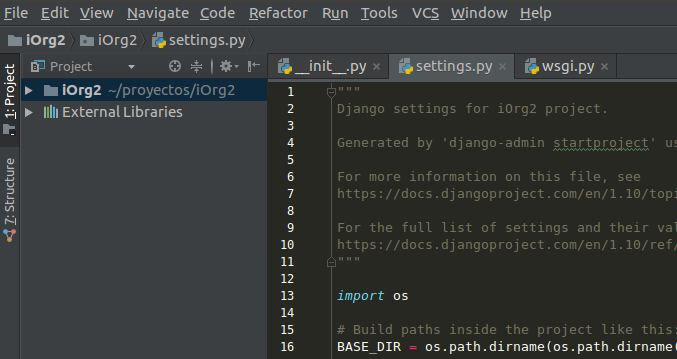
\includegraphics[width=0.6\textwidth]{../images/pycharm1.png}
  \caption[Pycharm 1/2]{ Captura de pantalla de la zona del proyecto }
  \label{fig:pycharm1}
  \end{center}
\end{figure}

\begin{figure}[!h]
  \begin{center}
  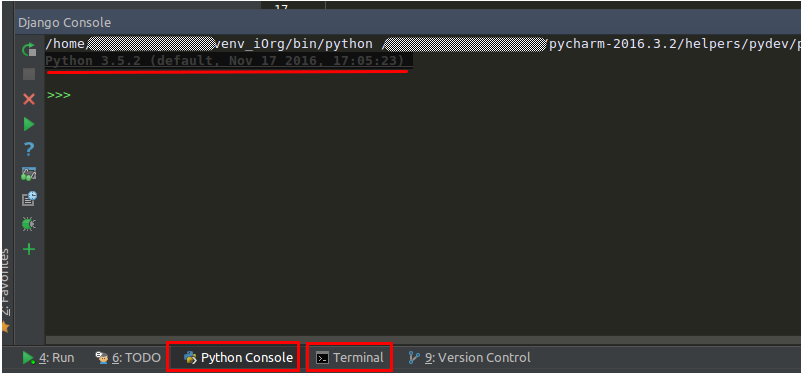
\includegraphics[width=0.6\textwidth]{../images/pycharm2.png}
  \caption[Pycharm 2/2]{ Captura de pantalla de la zona de la consola }
  \label{fig:pycharm2}
  \end{center}
\end{figure}

\bigskip
Además JetBrains\footnote{JetBrains: compañía desarrolladora de PyCharm (\href{https://www.jetbrains.com/}{https://www.jetbrains.com/})} ofrece el paquete profesional de PyCharm gratuito a estudiantes al que podemos acceder registrando nuestro correo de estudiante de la Universidad de Granada.

\bigskip 
Por las pruebas realizadas y las ventajas que ofrece vamos a utilizar PyCharm como IDE.



